\documentclass[a4paper]{article}
\usepackage[usenames,dvipsnames]{xcolor}
\usepackage{caption}
\usepackage{subcaption}
\usepackage{listings}
\usepackage{qtree}
\usepackage{xcolor}
\usepackage{forest}
\usepackage{multicol}
\setlength{\columnsep}{3cm}
\usepackage{parskip}
\usepackage{changepage}
\usepackage[T1]{fontenc}
\usepackage{amsmath}
\usepackage{hyperref}
\usepackage{listings}
\usepackage{amsthm}
\usepackage{amssymb}
\usepackage{float}
\usepackage[utf8]{inputenc}
\usepackage{graphicx}
\usepackage[italian]{babel}
\usepackage{thmtools}
\graphicspath{{figures/}}
\newtheorem*{definition}{Def}
\usepackage{xcolor}
\newcommand{\appunto}[1]{\textcolor{ForestGreen}{#1}}
\newcommand{\R}[0]{\mathbb{R}}
\newcommand{\C}[0]{\mathbb{C}}

\begin{document}

\author{Lorenzo Dentis, lorenzo.dentis@edu.unito.it}
\title{Numeri Complessi}
\maketitle
\section{definizione}
\begin{definition}
	Un numero complesso è una coppia ordinata $ (x,y) $ con $ x,y \in \mathbb{R} $.
	Nell' insieme dei numeri complessi $ \mathbb{C} = \{z = x + iy | x,y \in \mathbb{R}\} $ (posti $z_1,z_2 \in \mathbb{C}$) si definiscono le seguenti operazioni.
	\begin{itemize}
		\item[] \textbf{Addizione} $z_1+z_2 = (x_1+x_2, y_1 + y_2)$
		\item[] \textbf{Prodotto} $z_1z_2 = (x_1x_2 - y_1y_2,\; x_1y_2 + x_2y_1) $\\
			\appunto{La "formula" del prodotto si deduce facilmente da $(x_1 + iy_1) (x_2 + iy_2)$}
	\end{itemize}
\end{definition}
Un numero complesso può essere anche scritto in forma algebrica $z= x+iy$.
\begin{definition}
	Dato $z= (x,y)$ definisco "coniugato di $z$": $\overline z = (x,-y)$
\end{definition}
\section{proprietà}
Essendo un numero complesso una coppia di numeri reali, si può affermare $\mathbb{C} = \mathbb{R}^2$?\\
Sì,no,sì.\\ 
Insiemisticamente sono uguali \appunto{tanto che spesso si rappresentano i numeri immaginari sul piano di Gauss (piano complesso)} , $z$ è un punto in $\R^2$ di coordinate $(x,y)$
Algebricamente non sono uguali, in quanto il prodotto mostrato in $\mathbb{C}$ non è presente in $\mathbb{R}^2$.\\
La somma corrisponde alla somma di vettori in $\R^2$ ma il prodotto non ha corrispondenza.
\appunto{il prodotto vettoriale è  completamente diverso in $\mathbb{R}^2$.}\\
Topologicamente sono uguali, dato un numero complesso $z$, $||z|| = \sqrt{x^2 + y^2}$ chiamata \textit{norma} o \textit{modulo} di $z$. \appunto{cioè la stessa cosa del vettore di coordinate $(x,y) \in \R^2$}.
Da cui deriva che la "distanza" tra due numeri complessi $z,w$ è, \appunto{come in $\R^2$}, $dist(z,w)=||z-w|| = \sqrt{(x_z - x_w)^2 + (y_z - y_w)^2}$

Nota: il prodotto fornisce anche una giustificazione alle proprietà dell' \textit{unità immaginaria}
\begin{definition}
	$i=(0,1)$ è detta \textit{unità immaginaria} e verifica formalmente $i^2 =1$
\end{definition}
Infatti $i^2=(0,1)^2 = (0,1)(0,1) = (0*0 -1*1,0*1, 1 *0) = (-1,0) = 1$

\section{Altre forme di scrittura}
\subsection{Trigonometrica}
Rappresentando sul piano complesso un numero complesso $z$ notiamo che si può esprimere la sua "posizione" anche in coordinate polari.\\
\begin{figure}[H]
	\begin{subfigure}[c]{0.5\textwidth}
	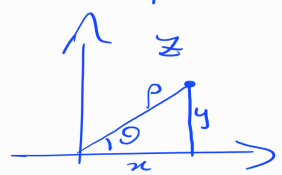
\includegraphics[width=\textwidth]{forma_trig.png}
	\end{subfigure}
	\begin{subfigure}[c]{0.5\textwidth}
		\begin{equation*}
			\begin{cases}
				\rho = \sqrt{x^2 +y^2}\\
				\theta = arctan(\frac{y}{x})
			\end{cases}
		\end{equation*}
		Vivecersa
		\begin{equation*}
			\begin{cases}
				x = \rho cos \theta\\
				y = \rho sin \theta
			\end{cases}
		\end{equation*}
	\end{subfigure}
\end{figure}
$$ z=x + iy = \rho\, cos \theta + i\,\rho \, sin \theta = \rho (cos\theta + i\,sin \theta)$$
Chiamiamo questo modo di esprimere un numero complesso "formai algebrica scritta in modo trigonometrico"

\subsection{Esponenzionale}
\begin{definition}[Formula di De Moivre]
	$$e^{i\theta} = cos\theta + i\, sen\theta$$
\end{definition}
Dunque
$$ z = \rho (cos \theta + sen \theta)=  \rho e^{i \theta}$$
\begin{definition}[Esponenziale complesso]
	In generale, sia $z = (x,y)$
	$$e^z = e^xe^{iy}=e^x(cos\,y + i \, sen\,x)$$
\end{definition}
La forma esponenziale permette di svolgere calcoli in maniera più semplice (soprattuto moltiplicazioni e potenze). 
\subsection{note}
Equivalenza tra la scrittura in forme algebrica e la scrittura come coppia di numeri reali.\\
$x = (x,0)\; y=(y,0),\; i=(0,1)$\\ 
$x+iy = (x,0) + (0,1)*(y,0) = (x,0) + (0*y - 1*0, 0*0 + 1*y ) = (x,0) + (0,y) = (x,y)$

Analisi a valori complessi:
Data un funzione $f: \mathbb{I} \rightarrow \C$,  $\forall t\in \mathbb{I},\; f(t)\in \C$
quindi può essere "scomposta": $f(t) = f_1(t) + i\,f_2(t)$.
\appunto{$f_1$ è la parte reale di $f_t$ ed $f_2$ la parte immaginaria}
\begin{definition}[Derivata a valori complessi]
	$$f'(t) = f_1'(t) + i\, f_2'(t)$$
\end{definition}
\begin{definition}[Integrale a valori complessi]
	$$\int_If(t) dt = \int_If_1(t) dt + i\, \int_If_2(t) dt$$
\end{definition}

\end{document}
